\documentclass[main.tex]{subfiles}
\begin{document}

\section{Linear methods}

\begin{figure}[H]
    \centering
    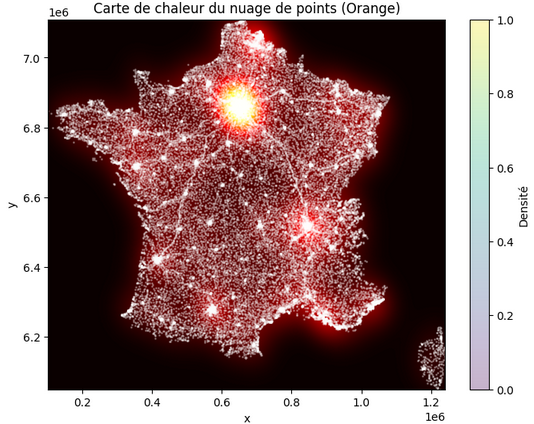
\includegraphics[width=0.7\textwidth]{Images/Heatmap_density_Orange.png}
    \caption{Heat map of the density}
\end{figure}

Generally, and as we can see on this heat map of the density of Orange base stations, roads are very dense areas. Therefore, we can try detecting them like we do for cities, using clustering per density. However, since we do not want the cities, we will consider that roads are dense clusters that are more elongated. To detect them, we will first apply a density clustering method, then keep only the clusters that are mostly linear using PCA. This is the same as removing clusters that are too non-linear, since cities are usually more round. 


\subsection{DBSCAN + PCA} 

This first try starts by detecting dense clusters with DBSCAN, before applying a PCA on each cluster, keeping only those which the first component explains most of the variance.

\textbf{Parameters : }
\begin{itemize}
    \item eps : used by DBSCAN, maximum distance for two points to be neighbors. Set to 6000 (meters) after a few tests and considering the mean distance between two points.
    \item min\_samples : used by DBSCAN, number of points to consider a neighborhood to be "dense". Set to 9 after a few tests and considering it as the least amount of stations for a road.
    \item explained\_thresh : a cluster is considered linear if its first PCA component is above this value. Set to 0.6 after tests.
\end{itemize}

\begin{figure}[H]
    \centering
    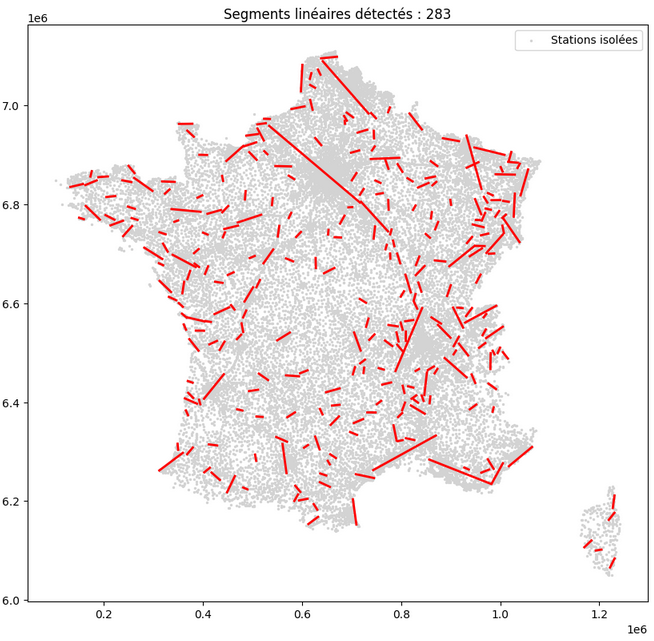
\includegraphics[width=0.6\textwidth]{Images/Res_DBSCAN+PCA.png}
    \caption{DBScan + PCA Result}
\end{figure}

\subsection{Tiles + PCA}

Considering the trouble detecting some portions of roads and suspecting it might be because some clusters corresponding to roads will be very long but not straight enough and thus rejected, this new method introduces tiles. The map is cut in squares, and we then determine if the points in the square are aligned using PCA as we did before. If the square is where a road is, the points inside it will be mostly aligned and thus we will trace the segment of road.

\textbf{Parameters : }
\begin{itemize}
    \item tile\_size : length of the tiles side. Set to 10 000 (meters) after a few tests, it should be rather small considering the goal is to see linear segments of roads and not their curves.
    \item min\_points : if there is less than this number of points, we consider it impossible to be part of a road and don't try PCA. It is very dependant of the previous parameter. Set to 6 after a few tests.
    \item min\_var\_ratio : a tile is considered linear if its first PCA component is above this value. Set to 0.6 considering the previous method.
\end{itemize}

\begin{figure}[H]
    \centering
    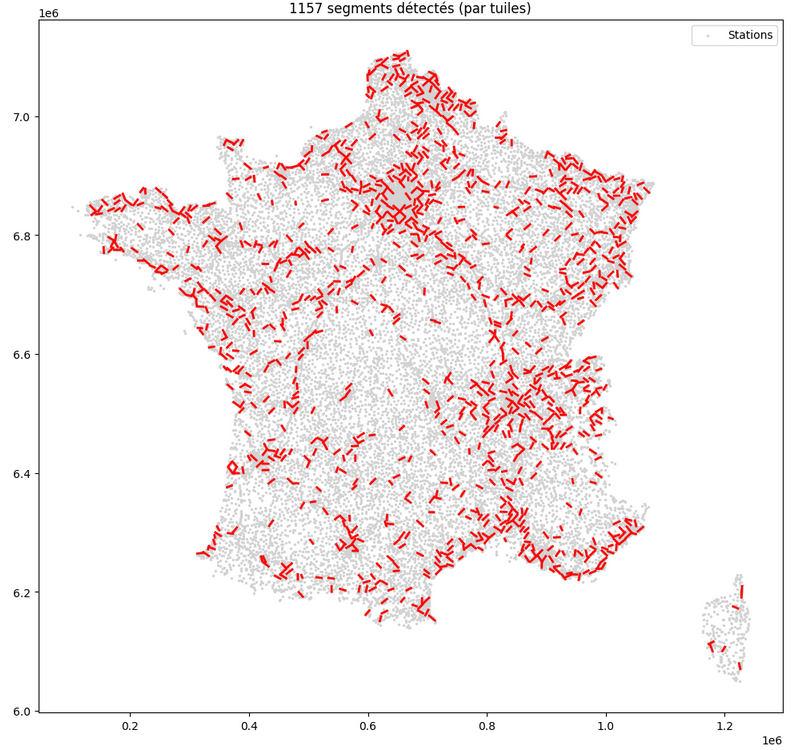
\includegraphics[width=0.6\textwidth]{Images/Res_Tiles+PCA.png}
    \caption{Tiles + PCA Result}
\end{figure}

This method does help with seeing where the detected roads are, and which segments are just noise. We also see the cities more clearly, since they are very dense in segments whereas for the previous method they caused some very long segments.

%%%%%%% KNN + PCA + clusters ???? %%%%%%%%

\subsection{Small conclusion}

These methods have reasonably good results, we can see some of the axes appearing, although there is also a lot of noise. However they also have a few problems : they detect the roads segment by segment, which means that we end up with very fractionated roads, and it makes the maps hard to read and distinguish the "right" segments from the noise. Moreover, here what we obtain is a mapping of the roads with segments, but we don't actually know which stations belong to these roads. What we would like is tracing the roads directly by linking the neighboring stations that are covering them.


\section{Aligned triplets method}

Since what we want to find is a following of stations that are mostly aligned, we try a different approach. This method uses triplets of stations that are aligned, and by concatenating them and keeping only the chains long enough and linear enough, we find the roads. 

We start by constructing a dictionary of aligned triplets : for each station, we consider its \textit{k} closest neighbors and for each pair of neighbors, if they are close enough (\textit{max\_dist}) and aligned enough (\textit{angle\_threshold}) with the station, then we save the triplet in the dictionary. Then, to construct the roads, we go through each triplet, and try to extend it by concatenating other triplets to it. 

\textbf{Parameters : }
\begin{itemize}
    \item k : number of neighbors to consider to construct the triplets. Set to 10 after a few tests.
    \item max\_dist : maximum distance to accept between stations in a chain/alongside a road. Set to 5500 after a few tests and considering the mean distance between two points.
    \item angle\_threshold : maximum angle accepted for a triplet to be considered aligned and kept. Going from 0 to 90 to measure the "flatness" of the angle. Set to 80 after a few tests, having it low removes too many possibilities (even when a segment of road is very straight, the stations covering it are not necessarily perfectly aligned).
    \item min\_chain\_length : minimal number of stations in a chain to keep it as a road. Set to 7 after a few tests, to minimize noise but keep as many roads sections as possible. 
\end{itemize}

\begin{figure}[H]
    \centering
    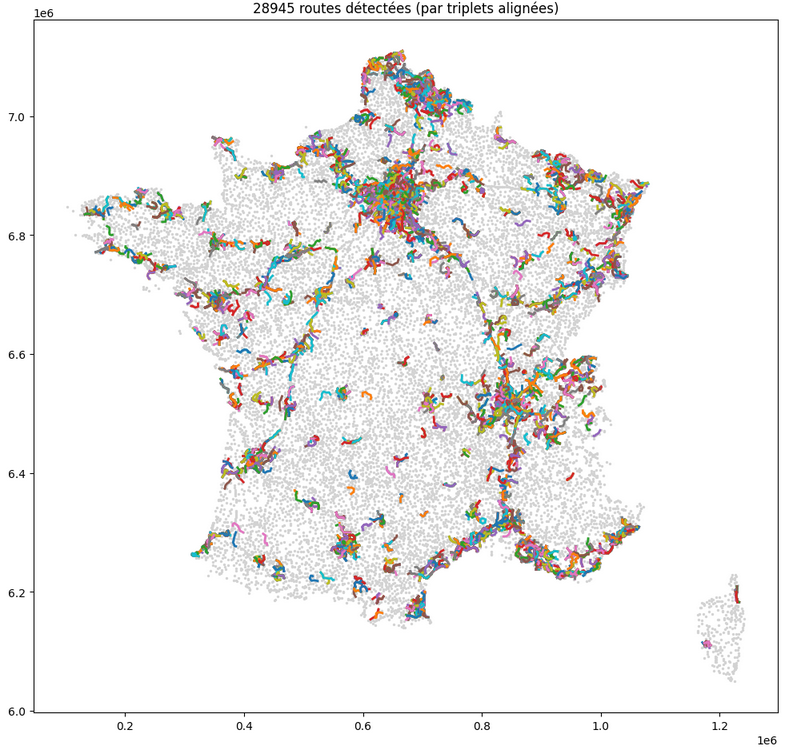
\includegraphics[width=0.7\textwidth]{Images/Res_Triplets.png}
    \caption{Triplets Result}
\end{figure}

\subsection{Triplets enhanced}

Seeing the time it takes to execute the method and the trouble it has to detect some road portions, we try a different approach. We now consider for every station each couple of neighbors (amongst the k nearest neighbors) and then verify if it is valid (they are close enough and aligned enough). Then instead of extending the chain by concatenating to it other triplets, we simply follow the direction of the initial triplet and consider the closest stations to continue the chain. Meaning, we consider the nearest neighbors of the station at the extremity of the chain. If the closest is close and aligned enough, we extend the chain with it, otherwise we consider the next neighbor. 

\textbf{Parameters : }
\begin{itemize}
    \item k : number of neighbors to consider to construct the triplets and extend the chains. Set to 10 after a few tests.
    \item dist\_max : maximum distance to accept between stations in a chain/alongside a road. Set to 5500 after a few tests and considering the mean distance between two points.
    \item angle\_max : maximum angle accepted for a triplet to be considered aligned and kept. Set to 40 after a few tests.
    \item angle\_max\_ext : maximum angle accepted to extend the chain. Set to 40 after a few tests.
    \item min\_chain\_length : minimal number of stations in a chain to keep it as a road. Set to 9 after a few tests, to minimize noise but keep as many roads sections as possible. 
\end{itemize}

\begin{figure}[H]
    \centering
    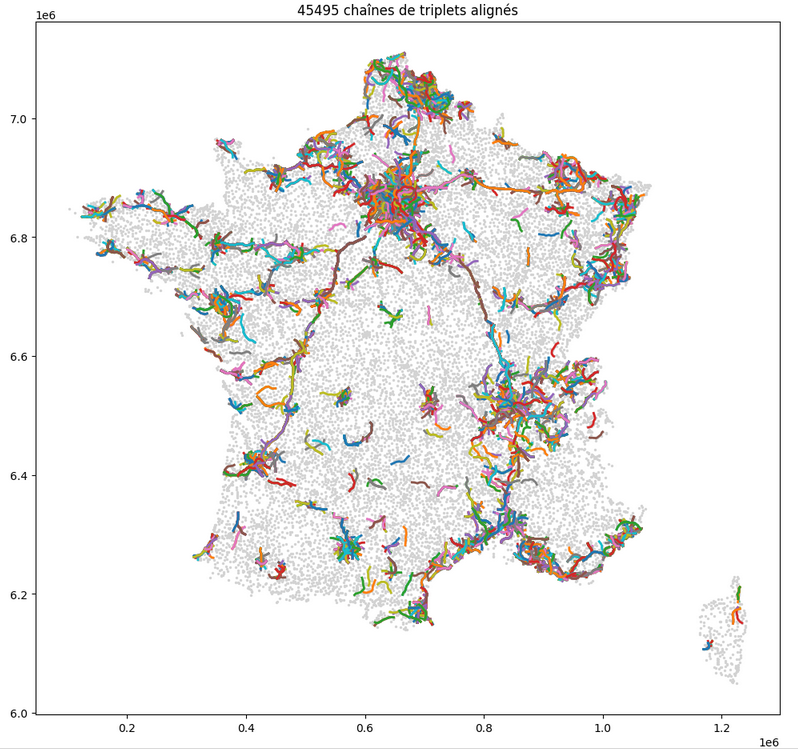
\includegraphics[width=0.7\textwidth]{Images/Res_Triplets_enhanced.png}
    \caption{Enhanced Triplets Result}
\end{figure}

We do obtain better results with this version of the method, and it takes less time to execute. However this method gives a lot of short chains, it would be better to obtain less but longer chains.



\section{Follow line method}

In search for even better results, detecting all the roads (we are still missing some east-west axis') with less noise and longer chains, here is another method, similar to how we extended the chains in the enhanced triplets method. 

For this method, we consider in turn every station as the start of a chain. We will go in \textit{n\_directions} from this point. To chose these directions, we consider the nearest base stations. We will keep the closest, if they are close enough and the directions are different enough (using \textit{angle\_tol}). Then each of these chains is extended using the same method as the previous : we add the closest station to the chain if it is close enough and aligned enough.

\textbf{Parameters : }
\begin{itemize}
    \item n\_neighbors : number of neighbors to consider to start and extend the chains. Set to 15 after a few tests.
    \item n\_directions : number of chains to try to start from a station. Set to 4 after a few tests. It is useless to go above 5. Setting it lower allows a faster execution but sometimes some roads are lost. Only going in one direction really misses a lot of roads.
    \item dist\_max : maximum distance to accept between stations in a chain/alongside a road. Set to 6000 after a few tests and considering the mean distance between two points.
    \item angle\_tol : minimum angle between starting directions. Set to 5 after a few tests. We can even let it be 0 if we consider that maybe we will find 2 different chains for the same road, but they are still both valid and removing one could mean losing some neighboring relations.
    \item angle\_max : maximum angle accepted to extend the chain. Set to 80 after a few tests and, as before, since stations will never be perfectly aligned.
    \item min\_len: minimal number of stations in a chain to keep it as a road. Set to 25 after a few tests, to minimize noise but keep as many roads as possible. It is longer here than for the previous methods since we do find longer chains and the shorter ones are mostly noise.
\end{itemize}

\begin{figure}[H]
    \centering
    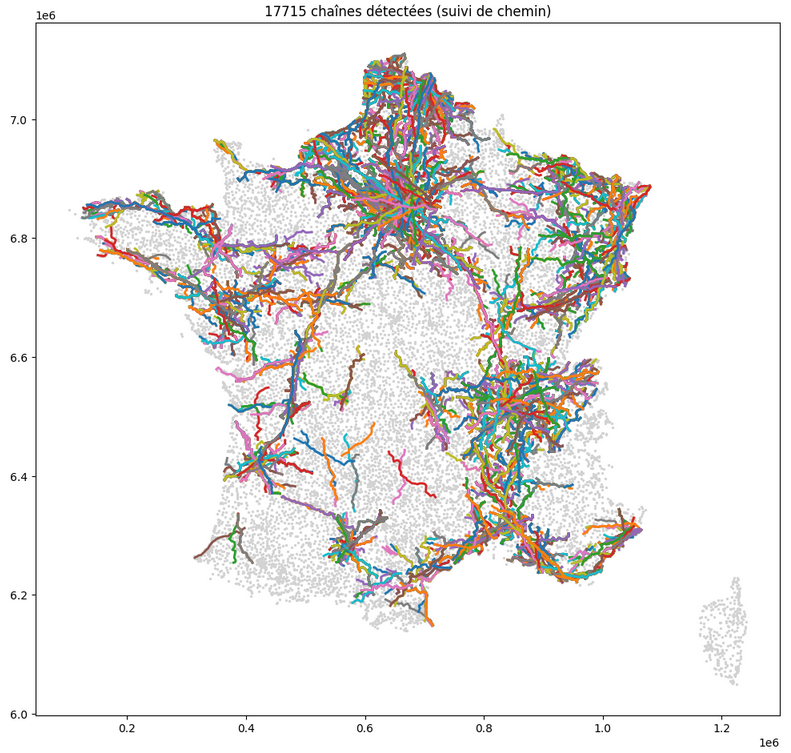
\includegraphics[width=0.7\textwidth]{Images/Res_Followline.png}
    \caption{Follow line result}
\end{figure}


\subsection{Parameters by density of roads}

With our methods we do not detect every department as well, in particular in most of the country's center we do not detect the roads at all. Thus we will try to adjust the parameters of this method according to the characteristics of the surroundings of a station. Usually, we can see that the departments containing mostly countryside are larger and contain less roads, while on the contrary departments containing big cities are smaller and have more roads. In the countryside we also often have less stations, which means we would need a longer distance between 2 stations alongside a road, whereas in cities we have a lot of stations thus they are closer. 

Hence for this version, we will use a ratio of length of roads over area for each department, to adjust our distance parameter accordingly. We first need to find some data : we need to know each department's surface, and the length of important roads and train tracks in it. For the surface, we use a data-set created last year putting together various information about the departments. We found a data-set for the roads and another for the train tracks on \href{https://www.observatoire-des-territoires.gouv.fr}{L'Observatoire des Territoires}, from 2010. 

Now, as said before, we will adjust the distance parameter according to this new ratio representing the density of roads in the department. To avoid having to set specific values to the parameter according to different values of the ratio, we will simply declare an interval for the distance, where the lowest value will have to be used where the density is high, and the highest will be used where the density is low. This replaces our previous \textit{dist\_max} parameter by \textit{dist\_min} and \textit{dist\_max}. The way the program chooses a value in this interval is as follow : it firstly calculates the density ratio for each department and normalizes it, before applying a linear transformation between it and our interval. Then we simply apply the follow line method department by department, changing the distance parameter accordingly. 

\textbf{Parameters : }
\begin{itemize}
    \item n\_neighbors : Set to 15 after a few tests.
    \item n\_directions : Set to 3 after a few tests. It is useless to go above 5. Setting it lower allows a faster execution but sometimes some roads are lost.
    \item angle\_tol : Set to 5 after a few tests. We can even let it be 0.
    \item dist\_min : Set to 1 after a few tests and considering the mean distance between two points.
    \item dist\_max : Set to 5500 after a few tests and considering the mean distance between two points.
    \item angle\_max : Set to 80 after a few tests and, as before, since stations will never be perfectly aligned.
    \item min\_len: Set to 9 after a few tests. It is lower here since we detect chains only by department, they will be shorter.
\end{itemize}

\begin{figure}[H]
    \centering
    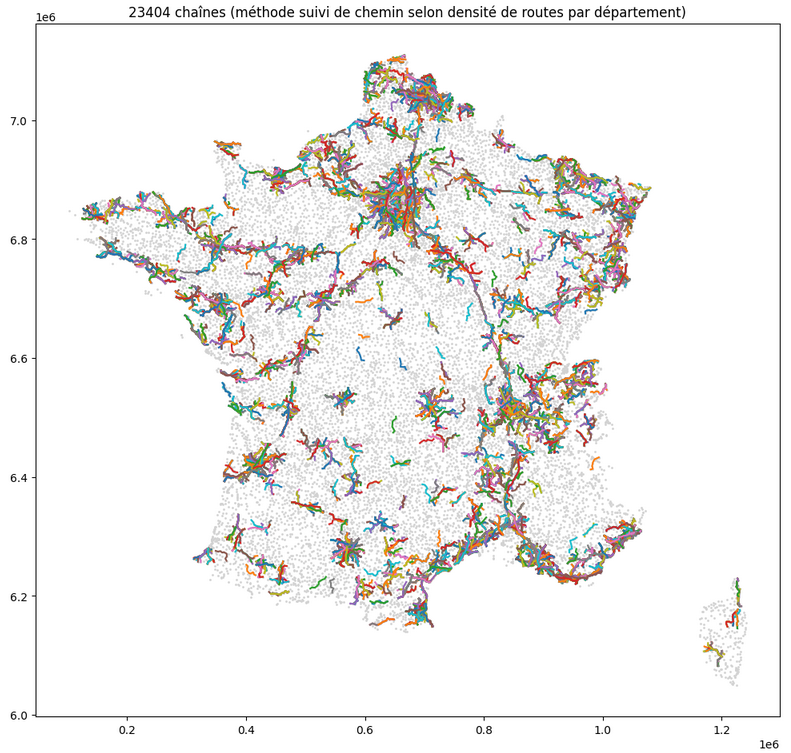
\includegraphics[width=0.7\textwidth]{Images/Res_Followline_Roaddens.png}
    \caption{Follow line by road density result}
\end{figure}


\subsection{Parameters by density of stations}

An even more adjusted method will be to use the density of stations in a radius around a station to decide which distance to use for this station. Indeed, if a station is part of a road and the density around it is very high, this means that the next station on the road is probably very close, whereas if the density is low, there will be more space between stations. This will be more adjusted and avoids separating the detection by departments. We will once again calculate for each station the density around it in a radius (\textit{r\_density}) and then normalize it. This time, we will adjust to it with a linear transformation the distance but also the angle (assuming that if there are less stations for a road they are also less aligned). This means we now have added a radius parameter and two intervals (4 parameters) instead of \textit{dist\_max} and \textit{angle\_max}.

\textbf{Parameters : }
\begin{itemize}
    \item n\_neighbors : Set to 15 after a few tests.
    \item r\_density : Set to 35 000 thinking about the area of Ile de France, which is the largest and most dense area of the map. 
    \item n\_directions : Set to 4 after a few tests. It is useless to go above 5. Setting it lower allows a faster execution but sometimes some roads are lost.
    \item angle\_tol : Set to 5 after a few tests. We can even let it be 0. 
    \item dist\_min : Set to 1 after a few tests and considering the minimum distance between two points.
    \item dist\_max : Set to 7000 after a few tests and considering the mean distance between two points.
    \item angle\_min : Set to 25 after a few tests.
    \item angle\_max : Set to 85 after a few tests.
    \item min\_len : Set to 40 after a few tests. We detect the longest roads with this method.
\end{itemize}

\begin{figure}[H]
    \centering
    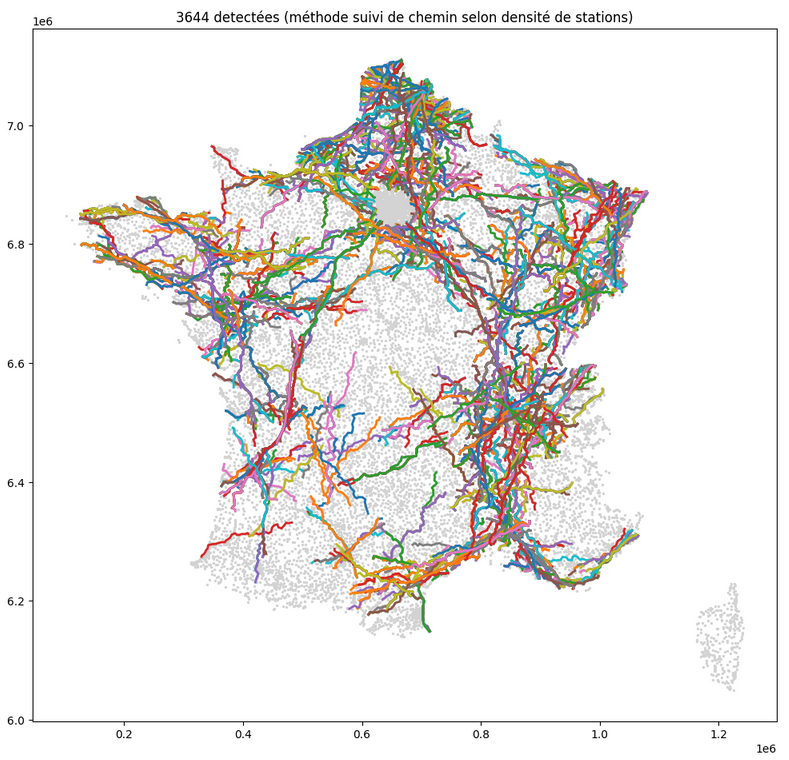
\includegraphics[width=0.7\textwidth]{Images/Res_Followline_Dens.png}
    \caption{Follow line by stations density result}
\end{figure}

We do manage to detect more roads with this method, which is the one that adapts to the territory the most. We can also obtain very different results by changing the parameters, for example sometimes we will see less chains for a road and less noise (here we have a lot of noise), but we will lose the Bordeaux-Lyon axis in most results. We will also probably have shorter chains. 


\end{document}